\section{Tunable Dimensions in the SZ Compression Pipeline}\label{sec:tunable dimensions}

In this section, we first review the general workflow of the SZ compression pipeline. We then identify the tunable configuration dimensions exposed by this pipeline and analyze their potential benefits and tuning costs under the hierarchical framework introduced in Section~\ref{sec:framework}, with the goal of determining appropriate tuning stages for different dimensions.

\subsection{SZ Compression Pipeline}

\begin{figure}[htb]
    \centering
    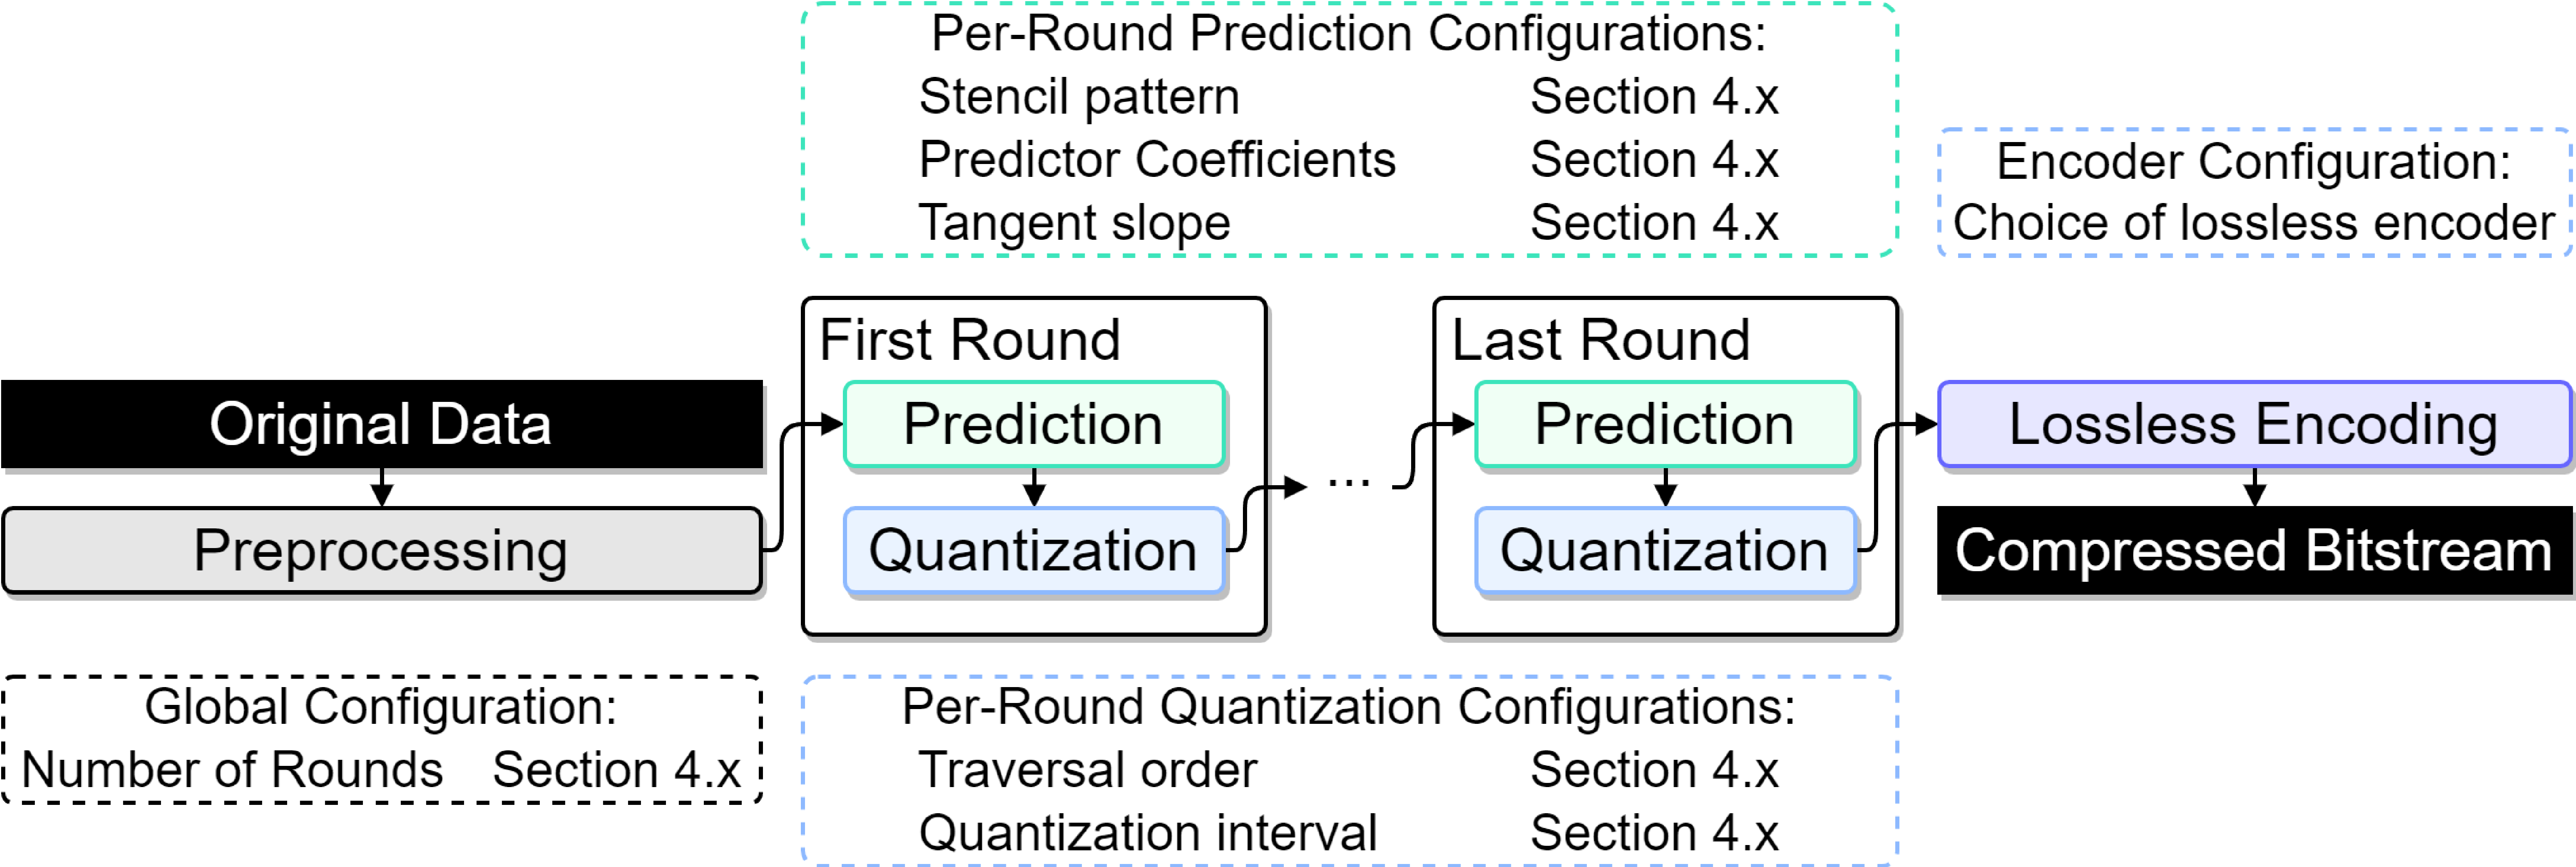
\includegraphics[width=1\linewidth]{figs/4/diagram2.pdf}
    \caption{Enter Caption}
    \label{fig:diagram2}
\end{figure}

The SZ compression pipeline mainly consists of three components: prediction, quantization of prediction residuals, and lossless encoding. As illustrated in Figure~\ref{fig:diagram2}, the prediction and quantization stages are divided into multiple rounds and executed iteratively. Each prediction round reconstructs a new set of data values, which can then serve as references in subsequent rounds. Lossless compression is applied only after the quantized residuals of all prediction rounds have been generated. The three components are described as follows.

\begin{itemize}
\item \textbf{Prediction.} A predictor commonly used in the SZ pipeline computes a weighted sum of selected reconstructed data points, referred to as \emph{reference points}, to estimate a data value that has not yet been reconstructed, referred to as the \emph{prediction target}. During decompression, the original data are unavailable, and the predictor can only access values that have already been reconstructed. Therefore, reference points must be selected exclusively from previously reconstructed data so that the compressor and decompressor can generate identical predictions. Such a weighted-sum predictor is characterized by a \emph{stencil pattern} and a set of \emph{coefficients}. The stencil pattern specifies the relative locations of the reference points with respect to the prediction target. The coefficients specify the weights assigned to the individual reference points.

Prediction is typically organized into multiple rounds. In each round, the number of newly predicted targets is approximately equal to the total number of values already reconstructed. Consequently, later rounds process progressively larger portions of the dataset and therefore have a substantially greater impact on the overall compression performance than earlier rounds.

\item \textbf{Quantization of prediction residuals.} For each prediction target, the compressor computes the difference between its original value and predicted value, and quantizes this residual to an integer multiple of the quantization interval $\Delta$. The quantized residual is then added to the prediction to obtain the reconstructed lossy value.

In the standard setting, choosing $\Delta=2\epsilon$, where $\epsilon$ is the user-specified error bound, guarantees pointwise error boundedness. However, a narrower quantization interval also preserves the error bound.

\item \textbf{Lossless compression.} After all prediction residuals have been quantized, the resulting integer symbols are losslessly encoded. Liu et al.~\cite{liu2021improving} showed that different lossless encoders can lead to different trade-offs between compression ratio and throughput. Their results indicate that Huffman coding followed by Zstandard compression provides moderate compression ratios while achieving the highest compression throughput. We therefore fix this encoding pipeline in ASZ and focus our configuration exploration on prediction and quantization.
\end{itemize}

\subsection{Tangent-Based Rate--Distortion Comparison}\label{sec:tunable dimensions:tangent}

The objective of error-bounded lossy compression is to achieve both a lower bit rate and higher reconstruction quality. However, a configuration change often introduces a trade-off between these two metrics: it may improve PSNR while increasing the bit rate, or reduce the bit rate at the cost of lower PSNR. Prior work by Liang et al.~\cite{liang2019significantly} compares configurations by adjusting their error bounds until they achieve the same bit rate or PSNR. Although this approach enables a direct comparison, it may require multiple additional compression runs.

\begin{figure}[htb]
    \centering
    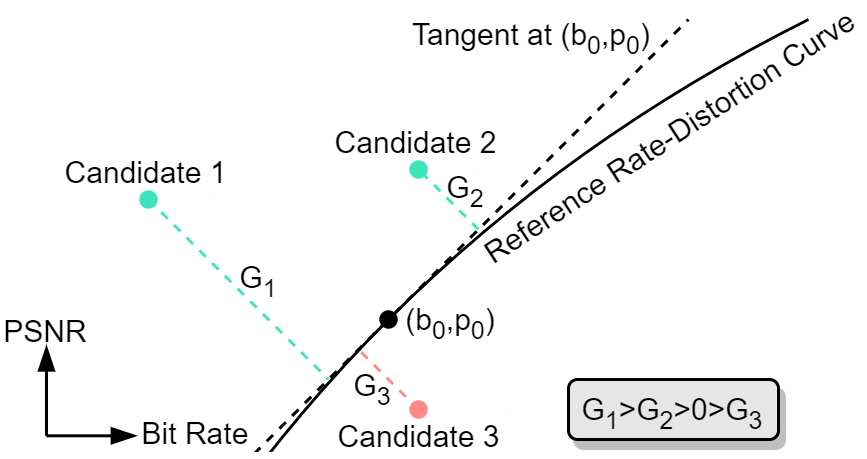
\includegraphics[width=0.7\linewidth]{figs/4/projection.png}
    \caption{Tangent-Based Rate--Distortion Comparison}
    \label{fig:tangent}
\end{figure}

To avoid this additional evaluation overhead, we propose a tangent-based rate--distortion comparison criterion, as illustrated in Figure~\ref{fig:tangent}. Given a reference configuration and a target error bound $eb_0$, we estimate the tangent of its rate--distortion curve at the corresponding operating point $(b_0,p_0)$, where $b_0$ denotes the bit rate and $p_0$ denotes PSNR. Specifically, we evaluate the reference configuration at two nearby error bounds on opposite sides of $eb_0$, namely, $eb_{\mathrm{low}}=eb_0/r$ and $eb_{\mathrm{high}}=eb_0r$, where $r>1$, obtaining the corresponding operating points $(b_{\mathrm{low}},p_{\mathrm{low}})$ and $(b_{\mathrm{high}},p_{\mathrm{high}})$. We approximate the local rate--distortion slope as
\begin{equation}
m_{\mathrm{RD}}=\frac{p_{\mathrm{high}}-p_{\mathrm{low}}}{b_{\mathrm{high}}-b_{\mathrm{low}}}.
\end{equation}

The estimated tangent at $(b_0,p_0)$ is expressed as
\begin{equation}
p-p_0=m_{\mathrm{RD}}(b-b_0).
\end{equation}

For a candidate configuration with operating point $(b_c,p_c)$ under the same error bound $eb_0$, we define its gain as the normalized signed offset from $(b_c,p_c)$ to the reference tangent:
\begin{equation}
G=\frac{p_c-p_0-m_{\mathrm{RD}}(b_c-b_0)}{\sqrt{1+m_{\mathrm{RD}}^2}}.
\end{equation}

A positive value of $G$ indicates that the candidate lies above the reference tangent, toward the preferred upper-left region of the rate--distortion plane, and therefore improves the local rate--distortion trade-off. $G=0$ indicates that the candidate moves only along the local rate--distortion trend. Therefore, candidates with larger values of $G$ are preferred.

\subsection{Analysis of Tunable Configuration Dimensions}\label{sec:tunable dimensions:analysis}

In the remainder of this section, we provide a more detailed explanation of the tunable configuration dimensions summarized in Figure~\ref{fig:diagram2}. For each dimension, we analyze its potential rate--distortion benefit, tuning costs and generalizability. Based on these factors, we determine the appropriate tuning stage within the hierarchical framework shown in Figure~\ref{fig:diagram1}. We first examine stencil patterns and predictor coefficients in Sections~\ref{aaa}---~\ref{bbb}, as these two dimensions are closely coupled and jointly determine the behavior of a predictor. We then analyze XXX.

\subsubsection{Tunable-Coefficient Predictors}\label{sec:tunable dimensions:analysis:TC predictor}\mbox{}

A weighted-sum predictor is jointly characterized by its stencil pattern and coefficients. The stencil pattern specifies the locations of the reference points relative to the prediction target, while the coefficients determine how these references are combined. In principle, a predictor may use reference points from a large neighborhood to exploit more information. In practice, however, only previously reconstructed values are available to both compression and decompression, and larger stencils increase computation costs. The stencil pattern therefore determines a restricted set of usable references.

\begin{figure}[htb]
    \centering
    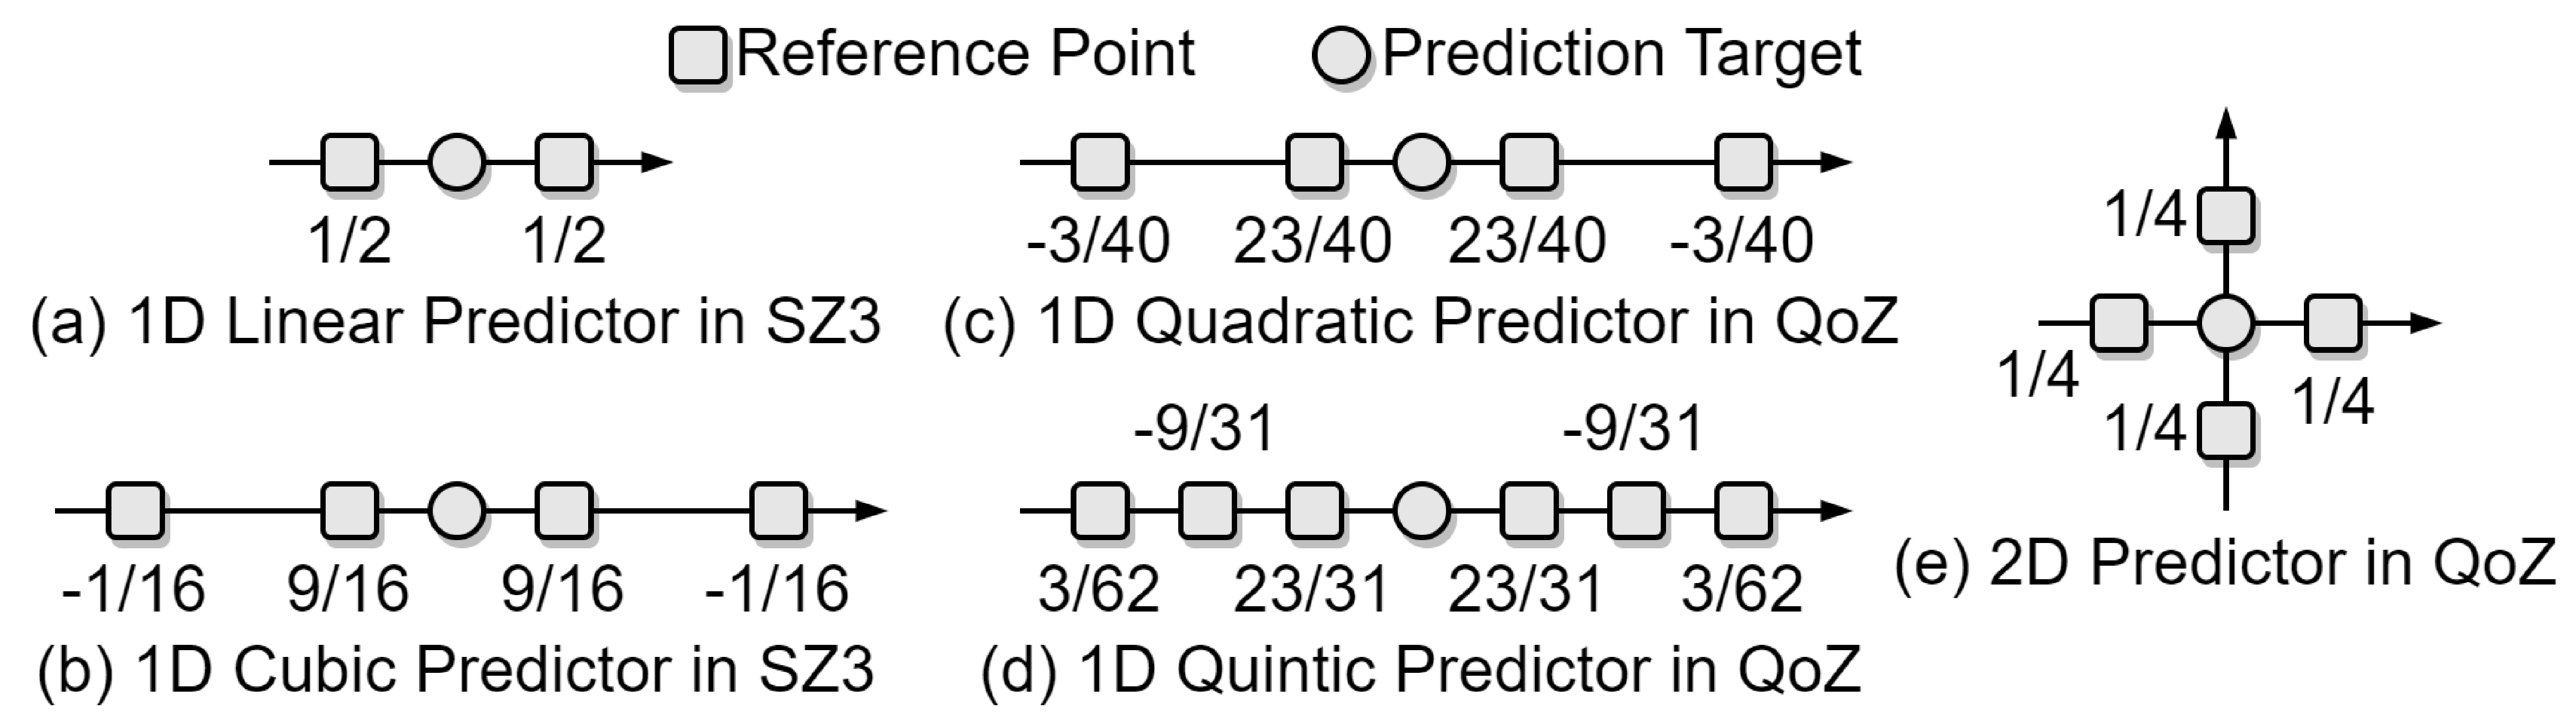
\includegraphics[width=1\linewidth]{figs/4/stencil patterns.pdf}
    \caption{Enter Caption}
    \label{fig:sp}
\end{figure}

Figure~\ref{fig:sp} illustrates several predictors used in SZ3 and QoZ. Additional predictors can be obtained by rotating these stencil patterns to align with different spatial dimensions. 

Both compressors include a predictor with four reference points along the same line (1D cubic predictor in SZ3 and 1D quadratic predictor in QoZ). However, they assign different coefficients to the same stencil pattern because they make different assumptions about local data behavior. SZ3 derives its coefficients by fitting a cubic polynomial through the four reference points, whereas QoZ constructs a piecewise quadratic spline under zero-slope boundary conditions. Other assumptions about local data characteristics can lead to different coefficient assignments. For example, under a stationary AR(1) correlation model, as the correlation parameter increases from $0$ toward $1$, the MSE-optimal coefficient assigned to each of the two reference points nearest to the prediction target increases from $0.25$ toward $0.5$. Meanwhile, the coefficients of the two outer reference points decrease from $0.25$ toward $0$. Notably, the coefficients assigned to the two inner reference points by SZ3 and QoZ are both greater than $0.5$, and therefore cannot be obtained under this stationary AR(1) model for any correlation parameter in $[0,1)$. These examples indicate that different assumptions about local data behavior lead to substantially different coefficient assignments, and no fixed coefficient assignment is uniformly optimal across different data characteristics.

Motivated by this observation, we define a ``tunable-coefficient predictor'' as a predictor with a fixed stencil pattern but adjustable coefficients. We constrain the coefficients to sum to one so that the prediction is exact for constant-valued data. Since all stencil patterns considered in this work are symmetric, coefficients at symmetric reference locations are constrained to be equal. When evaluating a tunable-coefficient predictor, we uniformly sample the feasible coefficient space and report the coefficient assignment that performs best under the tangent-based rate--distortion criterion introduced in Section~\ref{sec:tunable dimensions:tangent}.

\begin{figure}
    \centering
    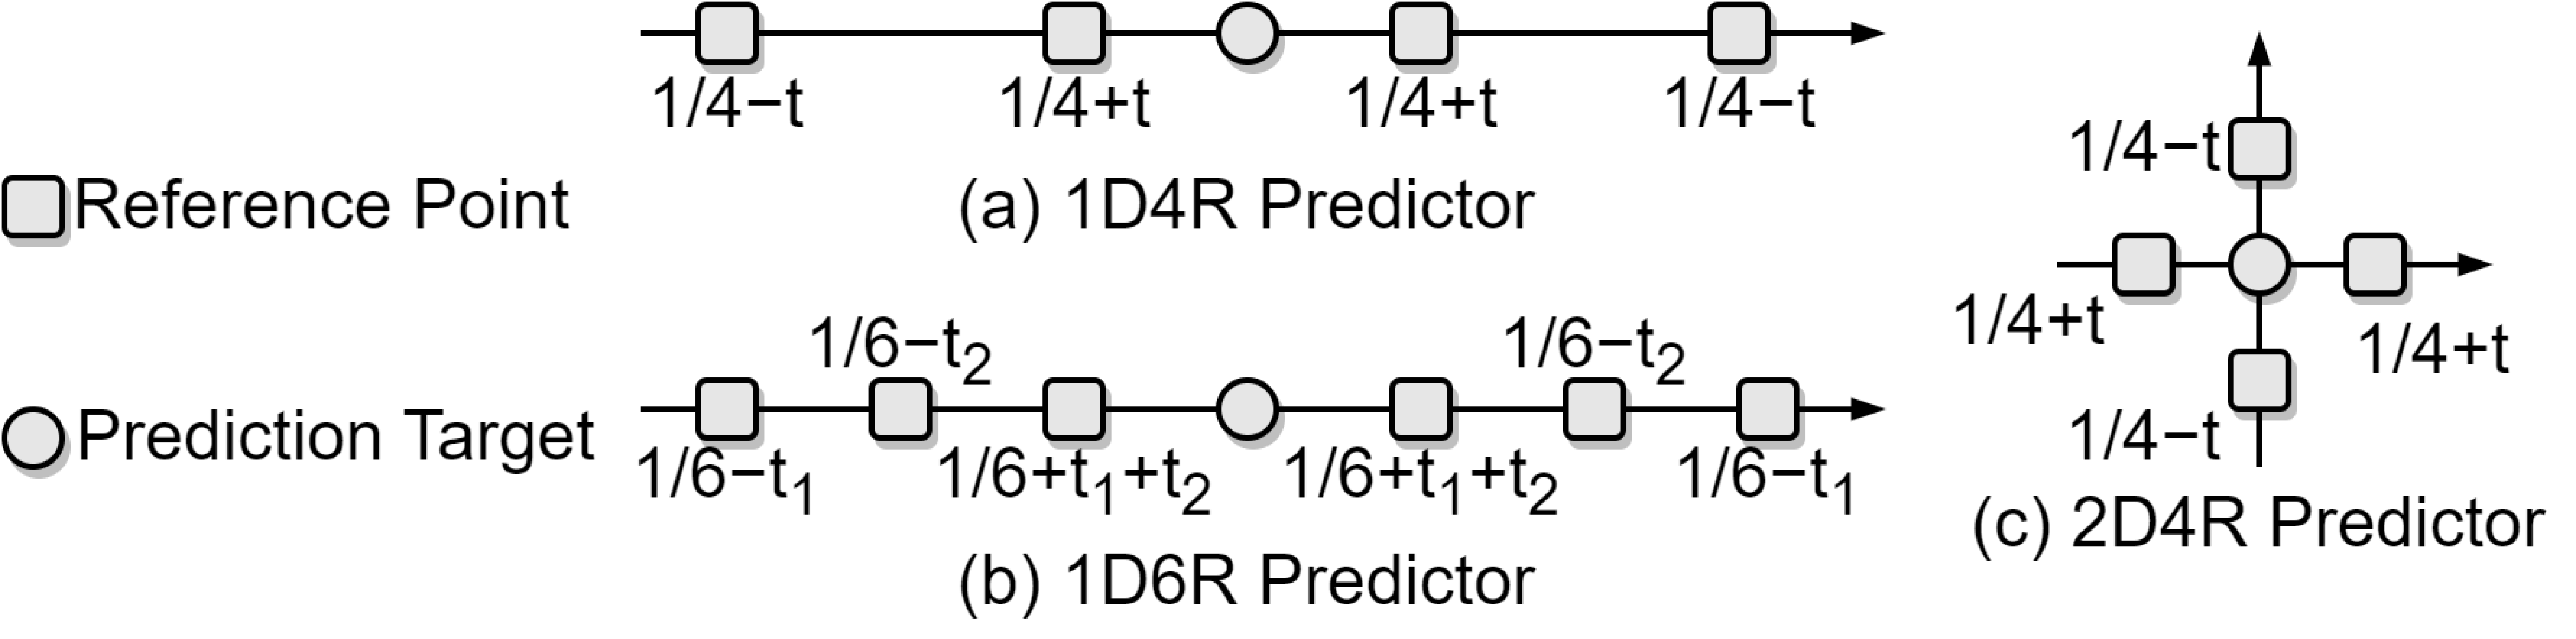
\includegraphics[width=1\linewidth]{figs/4/tunable coefficient stencil patterns.pdf}
    \caption{Enter Caption}
    \label{fig:tcsp}
\end{figure}

Predictors obtained by orienting the stencil geometry along different spatial directions form a predictor family. Figure~\ref{fig:tcsp} illustrates the three tunable-coefficient predictor families considered in this work. We use the notation $X$D$Y$R to denote a family whose predictors use $Y$ reference points distributed across $X$ spatial dimensions. 1D4R predictor family generalizes the linear and cubic predictors in SZ3 and the quadratic predictor in QoZ. Similarly, the 2D4R family generalizes the 2D predictor in QoZ, while the 1D6R family generalizes the quintic predictor in QoZ.

We evaluate the three tunable-coefficient predictor families on the ISABEL and CLDICE datasets in Table~\ref{tab:datasets}, and report their rate--distortion performance in Figure~\ref{fig:compare sp}. Both datasets are three-dimensional. Therefore, each predictor family can be instantiated along three orientations, corresponding to the three curves of the same color. The results lead to two main observations.

\begin{figure}[htb]
    \centering
    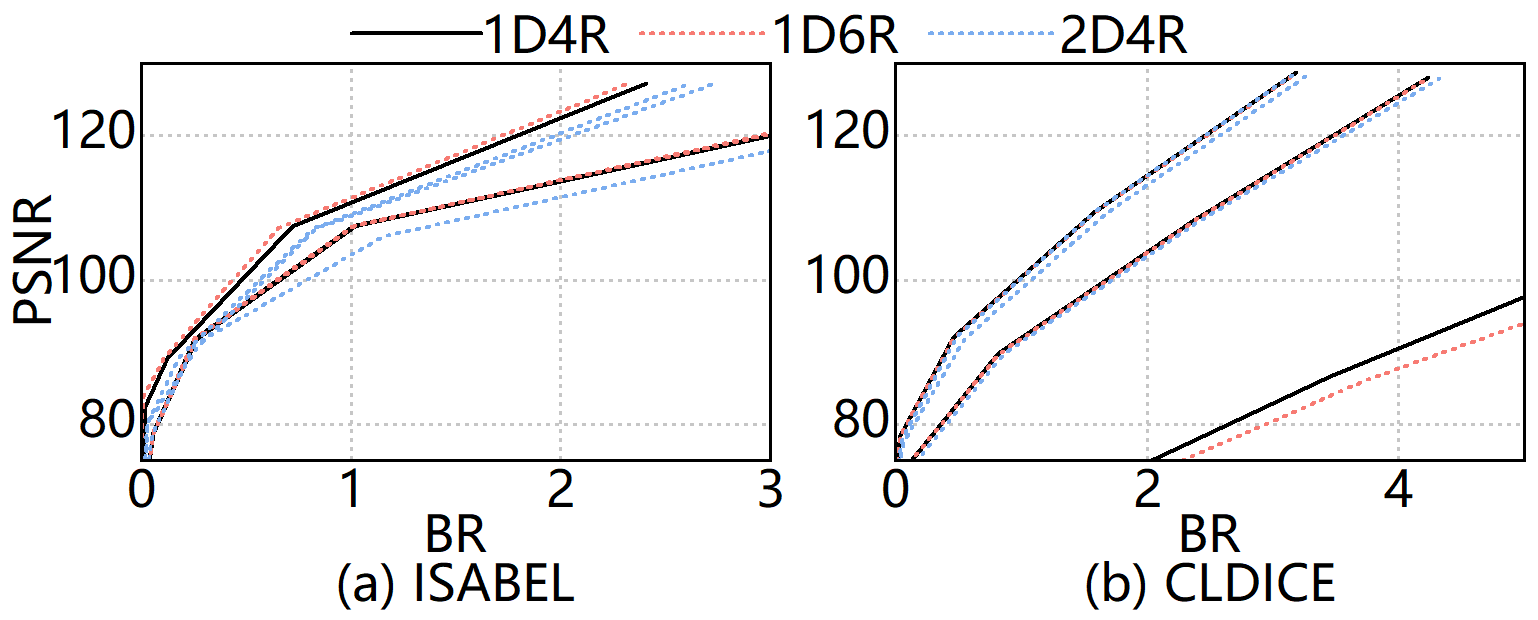
\includegraphics[width=0.8\linewidth]{figs/4/比较stencil pattern.png}
    \caption{Enter Caption}
    \label{fig:compare sp}
\end{figure}

\begin{itemize}
\item \textbf{The 2D4R predictors consistently underperform the 1D4R predictors.} After coefficient tuning, a 1D4R predictor can adaptively determine how much local nonlinear variation around the prediction target should be exploited. On noisy data, this information is often unreliable, and the optimal coefficients tend to approach those of the linear predictor in SZ3. On smoother data, the optimal coefficients tend to move toward those of the cubic predictor in SZ3 or the quadratic predictor in QoZ. This behavior suggests that the preferred 1D4R coefficients primarily reflect the overall usefulness of local nonlinear information, which is strongly influenced by the noise level and is often relatively consistent across a dataset.

In contrast, a 2D4R predictor can be viewed as a weighted combination of two one-dimensional linear predictions along different dimensions. Since neither component captures local nonlinear information, the resulting prediction errors contain unresolved nonlinear components from both directions. Appropriate coefficients may partially cancel these errors, but such cancellation is highly dependent on local data behavior and therefore does not generalize well across the dataset. This provides a possible explanation for the consistently weaker performance of 2D4R predictors.

\item \textbf{The improvement of 1D6R over 1D4R is very limited.} As shown in Figure~\ref{fig:compare sp}, the difference between the best 1D6R and 1D4R predictors is substantially smaller than the difference between the three oriented 1D4R predictors. Moreover, 1D6R introduces a larger coefficient-search space and incurs slightly higher prediction cost because it uses more reference points. We therefore exclude both 2D4R and 1D6R from the subsequent tuning space and retain 1D4R as the tunable-coefficient predictor family used in ASZ.
% 补充一下1D4R的参数搜索空间其实是1D6R的子集，所以最好的1D6R一定比最好的1D4R更好，但是优势非常少。
\end{itemize}

\subsubsection{Tuning Sequence of Stencil Patterns}\mbox{}

Existing compressors have explored tuning stencil patterns across prediction rounds, but only within restricted sequence structures. For three-dimensional data, SZ3 organizes every three consecutive rounds into a group, with the three rounds performing one-dimensional prediction along the three spatial dimensions, respectively. The prediction directions can be reordered within a group, but the same order is reused across all groups. QoZ expands this design by introducing two-dimensional predictors and allowing different groups to use different prediction orders. Nevertheless, both approaches retain the group structure and therefore explore only a restricted subset of possible prediction sequences.

We remove this grouping constraint and allow the differently oriented 1D4R predictors to be arranged freely across prediction rounds. The resulting search space grows exponentially with the number of rounds, making exhaustive evaluation impractical. We therefore adopt a backward greedy strategy that prioritizes the later prediction rounds. Specifically, we first select the stencil pattern for the final round and then proceed backward through the preceding rounds. Later rounds process substantially more prediction targets than earlier rounds and therefore generally have a greater impact on the overall rate--distortion performance. By fixing these high-impact choices first, the backward search provides an efficient approximation to exhaustive sequence tuning.

\begin{figure}[htb]
    \centering
    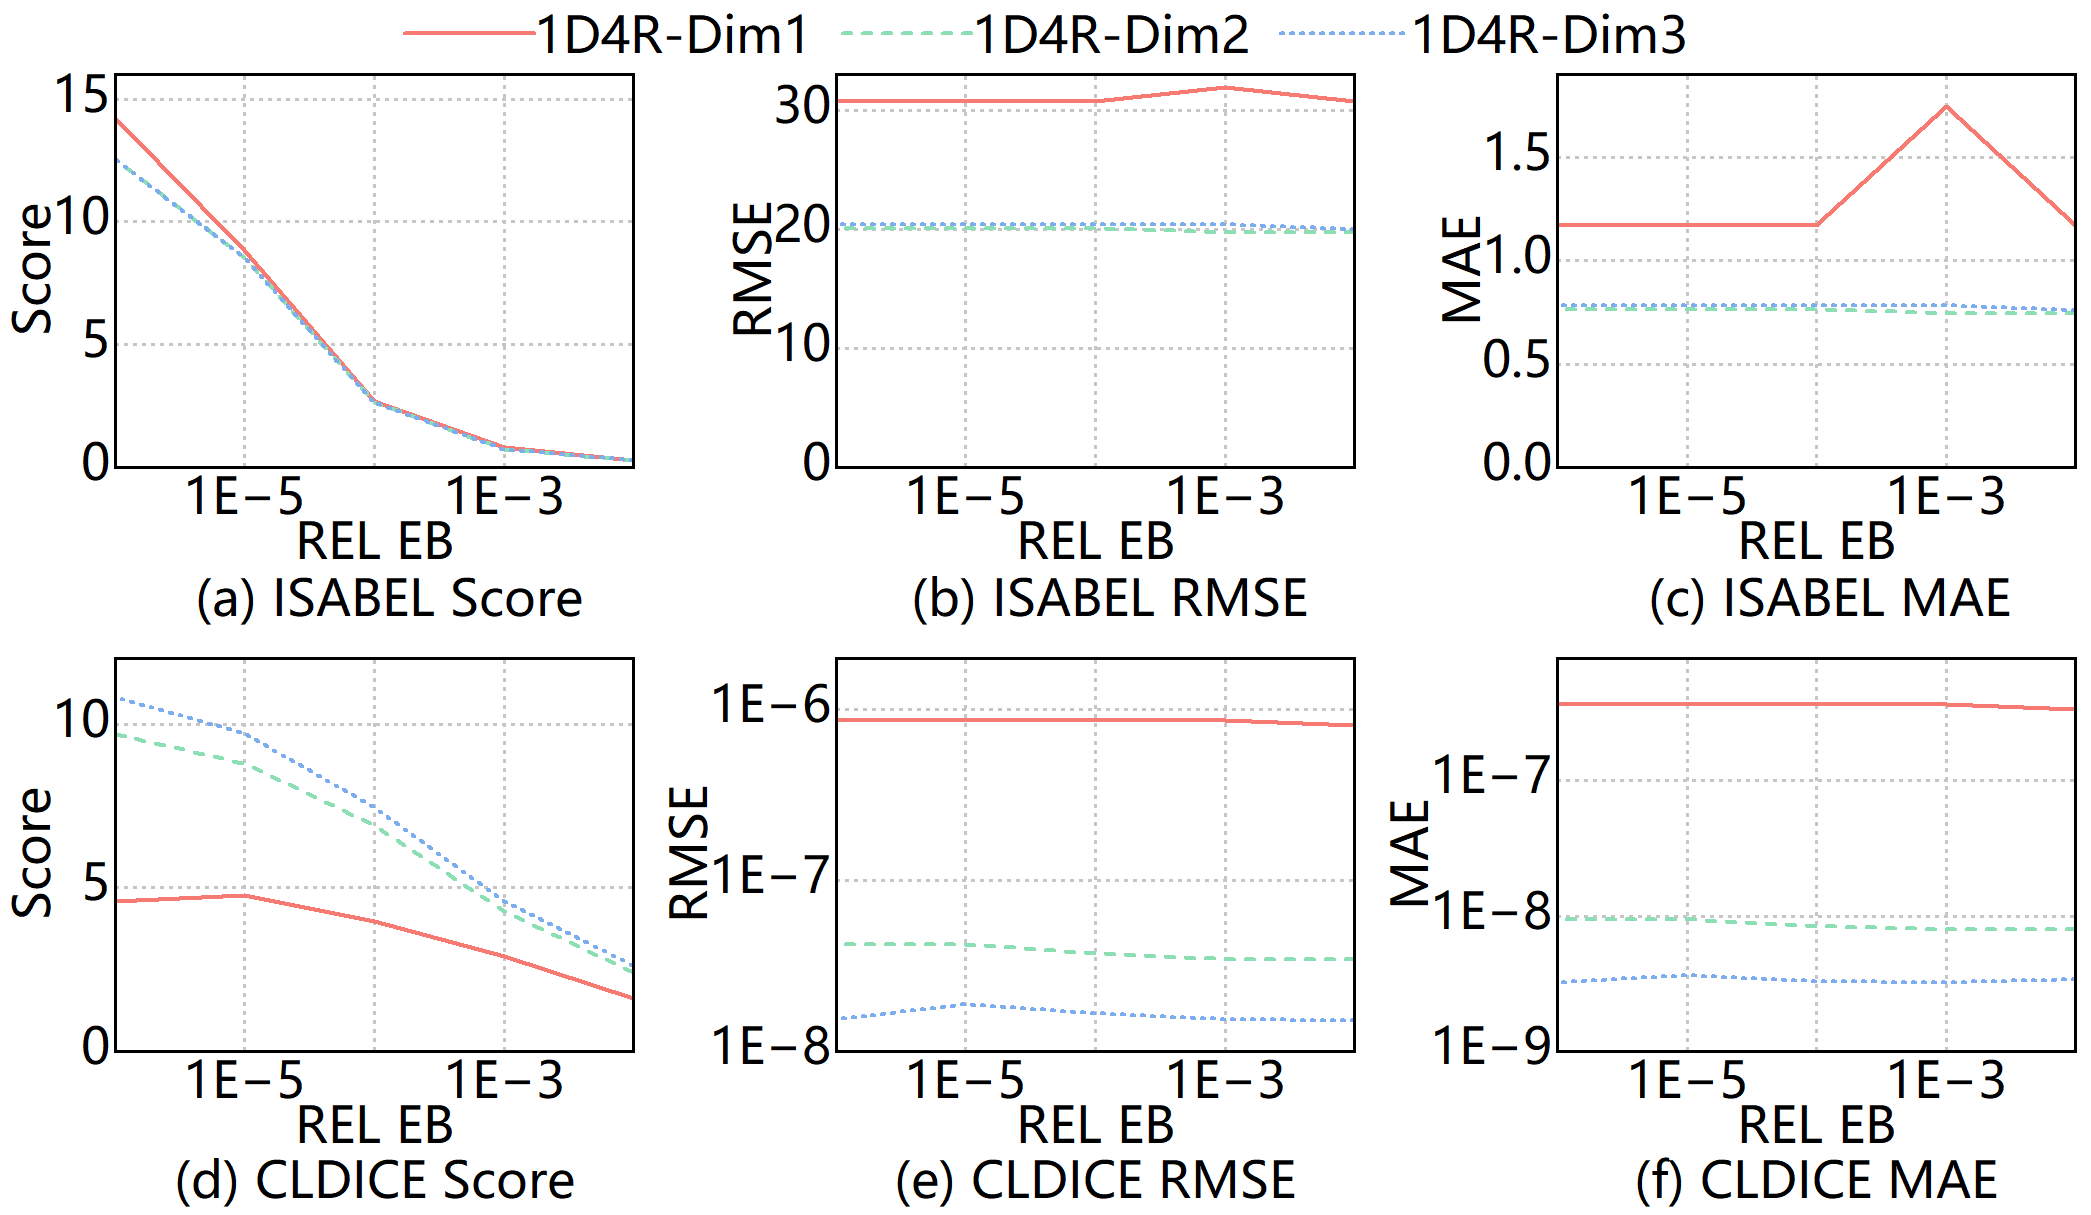
\includegraphics[width=1\linewidth]{figs/4/检验stencil pattern的proxy.png}
    \caption{Enter Caption}
    \label{fig:verify sp proxy}
\end{figure}

By comparing the solid black curves in Figure~\ref{fig:compare sp}, we observe that tuning the stencil pattern can provide significant rate--distortion improvement. However, we do not identify a reliable proxy for accelerating this tuning process.
Figure~\ref{fig:verify sp proxy} compares the tangent-based bit-rate--PSNR scores, prediction RMSE, and prediction MAE of the 1D4R predictors oriented along the three spatial dimensions on the ISABEL and CLDICE datasets. In principle, a well-performing predictor is expected to achieve a high rate--distortion score together with low prediction RMSE and MAE. However, this relationship is not consistently observed. On ISABEL, the predictor oriented along the first dimension achieves a high rate--distortion score despite also exhibiting high RMSE and MAE. Consequently, neither RMSE nor MAE reliably preserves the ranking of stencil candidates and therefore cannot serve as an effective proxy for stencil-pattern tuning. We further discuss the cause of this discrepancy in Section~\ref{sec:discussion}.

% 还要验证跨文件普适性

\subsubsection{Tuning Coefficients}\mbox{}

After selecting a 1D4R predictor, we further examine whether tuning its coefficients provides meaningful rate--distortion improvement. On the ISABEL and CLDICE datasets, we apply the best-performing 1D4R predictor identified in the preceding analysis and vary only its coefficient assignment. Figure~\ref{fig:bbb} compares the resulting rate--distortion curves.

The results show that different coefficient assignments can lead to substantial differences in rate--distortion performance. Moreover, the best-performing coefficients vary across datasets and error bounds, confirming that no single fixed assignment consistently achieves the best performance.

Predictor coefficients interact strongly with stencil patterns. Within the 1D4R family, predictors oriented along different dimensions may favor different coefficient assignments because the data can exhibit different characteristics along these dimensions. Therefore, when tuning stencil patterns, we must first identify the best coefficient assignment for each stencil candidate before comparing their rate--distortion performance. Since this process requires repeated evaluation of coefficient candidates, reducing the cost of each evaluation is essential for efficient stencil-pattern tuning.

\begin{figure}[htb]
    \centering
    \includegraphics[width=0.8\linewidth]{bbb}
    \caption{bbb}
    \label{fig:bbb}
\end{figure}

To reduce this cost, we replace the tangent-based bit-rate--PSNR comparison introduced in Section~\ref{sec:tunable-dimensions-tangent} with an $H_1$--PSNR comparison when ranking coefficient assignments for the same stencil predictor. Here, $H_1$ denotes the first-order entropy of the quantized prediction residuals and serves as an estimate of the bit rate. As shown in the first two columns of Figure~\ref{fig:bbb}, replacing bit rate with $H_1$ largely preserves the relative positions of the curves produced by different coefficient assignments, indicating that the $H_1$--PSNR comparison approximates the ranking obtained by the bit-rate--PSNR comparison.

The third column of Figure~\ref{fig:bbb} compares the ranking accuracy of five inexpensive evaluation criteria: the proposed $H_1$--PSNR criterion, $H_1$ alone, PSNR alone, prediction MSE, and prediction MAE. The horizontal axis shows the relative error bound, while the vertical axis reports Kendall's $\tau$ between the candidate ranking produced by each criterion and the ranking produced by the bit-rate--PSNR criterion. Across the evaluated error bounds, the $H_1$--PSNR criterion achieves the highest ranking accuracy.

Compared with the original bit-rate--PSNR criterion, the $H_1$--PSNR criterion first reduces the evaluation cost by eliminating lossless encoding. Both $H_1$ and PSNR can be obtained while computing the quantized prediction errors: $H_1$ is calculated from the resulting symbol distribution, while PSNR is derived from the corresponding reconstruction errors.

A direct evaluation of the $H_1$--PSNR criterion processes each coefficient candidate independently. For each candidate, it predicts all sampled target values, quantizes the resulting prediction errors, counts the frequencies of the quantization symbols to compute $H_1$, and accumulates the reconstruction errors to compute PSNR. Although this approach avoids the lossless-encoding stage required by the bit-rate--PSNR criterion, it still requires prediction and quantization for every combination of coefficient candidate and sampled target.

The evaluation can be further accelerated without explicitly computing and quantizing the prediction error of every sampled target for every coefficient candidate. Both $H_1$ and PSNR depend only on the distribution of prediction errors, rather than on their spatial ordering. Therefore, once an accurate approximation of this distribution is available, the frequencies of the quantized prediction-error symbols and the resulting PSNR can be estimated directly using the following equations.

Let the prediction error $E$ follow a probability density function $f_E(e)$, and let $\Delta$ denote the quantization step size. Under uniform quantization, the probability of quantization symbol $i$ is
\begin{equation}
p_i=\int_{\left(i-\frac{1}{2}\right)\Delta}^{\left(i+\frac{1}{2}\right)\Delta}f_E(e)\,de.
\end{equation}
The first-order entropy is then computed as
\begin{equation}
H_1=-\sum_i p_i\log_2p_i.
\end{equation}
Because an error in the $i$th interval is reconstructed as $i\Delta$, the resulting mean squared reconstruction error is
\begin{equation}
\mathrm{MSE}_{\mathrm{rec}}=\sum_{i=-\infty}^{\infty}\int_{\left(i-\frac{1}{2}\right)\Delta}^{\left(i+\frac{1}{2}\right)\Delta}f_E(e)\left(e-i\Delta\right)^2\,de.
\end{equation}
The corresponding PSNR is
\begin{equation}
\mathrm{PSNR}=10\log_{10}\left(\frac{R^2}{\mathrm{MSE}_{\mathrm{rec}}}\right),
\end{equation}
where $R$ is the value range of the original data.


为了快速算出预测误差的分布，We exploit this property by expressing the prediction error as an affine function of the tunable coefficient. For the 1D4R predictor shown in Figure~\ref{fig:tcsp}, the prediction error for a target $x_0$ can be written as
\begin{equation}
e(t)=x_0-\left[\left(\frac{1}{4}-t\right)x_{-3}
+\left(\frac{1}{4}+t\right)x_{-1}
+\left(\frac{1}{4}+t\right)x_1
+\left(\frac{1}{4}-t\right)x_3\right]
=At+B,
\end{equation}
where
\begin{equation}
A=x_{-3}-x_{-1}-x_1+x_3
\end{equation}
and
\begin{equation}
B=x_0-\frac{x_{-3}+x_{-1}+x_1+x_3}{4}.
\end{equation}

The values of $A$ and $B$ are independent of the coefficient candidate $t$. We therefore compute them once for all sampled prediction targets and construct an approximate joint histogram of $(A,B)$. For a candidate $t$, each occupied histogram bin centered at $(a_j,b_j)$ is mapped to the prediction error $a_jt+b_j$. After quantizing these errors under the target error bound and aggregating the corresponding bin frequencies, we directly obtain an approximation of the quantized-error distribution used to compute $H_1$ and PSNR. This avoids recomputing the prediction error separately for every sampled target and every coefficient candidate.

Let $n$ be the number of sampled prediction targets, $k$ the number of coefficient candidates, and $h$ the number of occupied bins in the joint histogram of $(A,B)$. Direct evaluation computes an error for every target--candidate pair and therefore requires $O(kn)$ time. The histogram-based method requires $O(n)$ time to construct the joint histogram and $O(kh)$ time to evaluate all candidates, resulting in a total complexity of $O(n+kh)$. Since $h$ is typically much smaller than $n$, the evaluation cost is close to linear in the sample size.

The joint histogram need not preserve $A$ and $B$ at full numerical precision. The final $H_1$ calculation only distinguishes prediction errors after quantization, whose interval is determined by the error bound. Therefore, the discretization intervals used for $A$ and $B$ can be substantially smaller than, but need not be comparable to machine precision relative to, the final prediction-error quantization interval. In our implementation, setting their induced error uncertainty to a small fraction of the final quantization interval, such as $10\%$, is sufficient to preserve an accurate quantized-error distribution.

Moreover, the expressions for $A$ and $B$ represent local differences and interpolation residuals, respectively, and are therefore typically concentrated near zero for locally correlated scientific data. As a result, only a limited number of joint-histogram bins are occupied in practice, making $h\ll n$ and reducing the overall evaluation cost to approximately $O(n)$ for a fixed set of coefficient candidates.